% ============================================================
%  chapter05_variations_on_ctw_slides.tex
%  Chapter 5: Variations on CTW
%  An Introduction to Universal Artificial Intelligence
%  Hutter, Quarel & Catt --- CRC Press, 2024
% ============================================================
\documentclass[aspectratio=169,10pt]{beamer}

\usetheme{Madrid}
\usecolortheme{seahorse}
\usefonttheme{professionalfonts}

% -- packages ------------------------------------------------------------------
\usepackage{amsmath,amssymb,bm}
\usepackage{stmaryrd}
\usepackage{graphicx}
\usepackage{booktabs}
\usepackage{listings}
\usepackage{xcolor}
\usepackage{tikz}
\usetikzlibrary{shapes,arrows,positioning,calc}
\usepackage{mathtools}
\usepackage{array}
\usepackage{multirow}
\usepackage{makecell}
\usepackage{algorithm}
\usepackage{algpseudocode}

\graphicspath{{figures/}}

% -- listings style --------------------------------------------------------
\lstdefinestyle{pythonstyle}{
  language=Python,
  basicstyle=\ttfamily\scriptsize,
  keywordstyle=\color{blue}\bfseries,
  stringstyle=\color{orange},
  commentstyle=\color{green!50!black}\itshape,
  numberstyle=\tiny\color{gray},
  numbers=left,
  stepnumber=1,
  numbersep=5pt,
  frame=single,
  backgroundcolor=\color{gray!7},
  breaklines=true,
  showstringspaces=false,
  tabsize=2,
  captionpos=b,
}
\lstset{style=pythonstyle}

% -- beamer setup -----------------------------------------------------------
\setbeamertemplate{footline}[frame number]
\setbeamertemplate{navigation symbols}{}
\setbeamersize{text margin left=0.5cm, text margin right=0.5cm}

% -- convenient macros -------------------------------------------------------
\newcommand{\Bstr}{\mathbb{B}^*}
\newcommand{\explain}[1]{\par\smallskip{\footnotesize\itshape #1}\par}
\newcommand{\KT}{\mathrm{KT}}
\newcommand{\CTW}{\mathrm{CTW}}
\newcommand{\CTS}{\mathrm{CTS}}
\newcommand{\PTW}{\mathrm{PTW}}
\newcommand{\FMN}{\mathrm{FMN}}

% -- title -------------------------------------------------------------------
\title[UAI -- Ch.5 Variations on CTW]{An Introduction to Universal Artificial Intelligence}
\subtitle{Chapter 5: Variations on CTW}
\author{Based on Hutter, Quarel \& Catt}
\institute{CRC Press, 2024}
\date{}

% =============================================================================
\begin{document}
% =============================================================================

\begin{frame}
  \titlepage
  \begin{center}
  \footnotesize\itshape ``If you can't program it, you haven't understood it.'' --- David Deutsch
  \end{center}
\end{frame}

\begin{frame}{Outline}
  \tableofcontents
\end{frame}

% =============================================================================
\section{5.0 Recap and Roadmap}
% =============================================================================
\begin{frame}[allowframebreaks]{Where We Left Off: CTW}
  In Chapter 4 we saw that \textbf{Context Tree Weighting (CTW)} is an
  efficient method for computing a Bayesian mixture $\mathrm{P}_D^{\CTW}$
  (Definition 4.5.4) over a class $\mathcal{M}$ of variable-order Markov
  sources. If the true distribution $\mu$ (mu) is $k$-Markov (its next symbol
  depends only on the previous $k$ symbols), CTW learns to predict well, and
  does so in time and space that scale only polynomially in the sequence
  length and the maximum depth $D$.

  \medskip
  CTW rests on one standing assumption: the source is \textbf{stationary} --
  the distribution over $x_t$ depends on the preceding symbols
  $x_{t-k},\dots,x_{t-1}$ but never on the time index $t$ itself. This
  chapter weakens that assumption along several different axes, giving four
  variations on CTW:

  \begin{itemize}
    \item \textbf{Adaptive CTW} (\S5.1): replace the KT estimator with a
      \emph{discounted} version that forgets old data, so CTW can track
      slowly drifting (non-stationary) sources.
    \item \textbf{Context Tree Switching (CTS)} (\S5.2): mix over
      \emph{sequences} of PST models rather than a single fixed model,
      allowing abrupt regime changes.
    \item \textbf{Partition Tree Weighting (PTW)} (\S5.3): mix over
      \emph{partitions of time} rather than contexts, for piecewise
      stationary sources.
    \item \textbf{Forget-Me-Not (FMN)} (\S5.4): a meta-algorithm generalizing
      PTW with a memory of past model states, for repeating non-stationary
      sources.
  \end{itemize}
  We finish with \textbf{Context Tree Maximization (CTM)} (\S5.5), which
  replaces CTW's Bayesian \emph{mixture} over trees with a single
  \emph{maximum a posteriori} (MAP) tree -- an instance of the Minimum
  Description Length principle.
\end{frame}

% =============================================================================
\section{5.1 Adaptive CTW}
% =============================================================================

\begin{frame}[allowframebreaks]{Motivation: CTW Assumes Stationarity}
  The CTW method operates under the assumption that the true distribution is
  \textbf{stationary}: the distribution over $x_t$ depends only on previous
  terms $x_{t-k},x_{t-k+1},\dots,x_{t-1}$, and \emph{not} on the current time
  step $t$. This makes the \textbf{KT estimator} (Krichevsky--Trofimov
  estimator, Lemma 4.1.2 -- a simple Bayesian estimator for the bias of a
  coin) an appropriate choice: it takes into account \emph{all} statistics
  observed so far and assigns \emph{equal} weight to old and recent samples.

  \medskip
  For \textbf{non-stationary} sources, the KT estimator is a poor choice. As
  more samples are collected, the contribution of each new symbol to the
  running counts becomes smaller relative to the accumulated total, making
  it difficult to detect changes or shifts in the distribution over time. To
  fix this we need to replace the KT estimator with one that places more
  weight on \emph{recent} data, while keeping CTW's computational
  efficiency. This is the idea of \textbf{Adaptive CTW} [OHSS12]: use a
  \emph{discounted} KT estimator that assigns higher weight to more recent
  data, similar to how rewards are discounted in reinforcement learning
  (Section 6.4).

  \framebreak

  \textbf{Standard KT counts.} For the standard KT estimator, counts $a$ and
  $b$ are incremented whenever a zero or a one is observed, respectively.
  Writing $a_t,b_t$ for the counts after observing $x_{1:t}$, the update
  rule is
  \[
    a_{t+1} = \llbracket x_{t+1}=0\rrbracket + a_t, \qquad
    b_{t+1} = \llbracket x_{t+1}=1\rrbracket + b_t.
  \]
  \explain{Here $\llbracket \cdot \rrbracket$ is the indicator function (1 if
  the statement inside is true, 0 otherwise). So $a_t$ is simply the number
  of 0s seen so far and $b_t$ the number of 1s seen so far -- every past
  observation counts exactly once, forever.}

  \textbf{Discounted KT counts.} We introduce a \textbf{discount}
  $\gamma$ (gamma), $\gamma\in[0,1]$, that controls how quickly old counts
  decay: the larger $\gamma$, the faster the decay. The increments are still
  made based on the newly observed value, after which the \emph{whole} count
  is scaled down by $(1-\gamma)$:
  \[
    a_{t+1} = (1-\gamma)\big(\llbracket x_{t+1}=0\rrbracket + a_t\big), \qquad
    b_{t+1} = (1-\gamma)\big(\llbracket x_{t+1}=1\rrbracket + b_t\big).
  \]
  \explain{Every time step, the accumulated counts $a_t,b_t$ are shrunk by
  the factor $(1-\gamma)$ \emph{before} being used again, so an observation
  from $n$ steps ago contributes only $(1-\gamma)^n$ as much as a fresh
  observation. If $\gamma=0$ this reduces exactly to the standard
  (undiscounted) KT estimator. Note $\gamma$ need not be a constant -- it can
  be parameterized in different ways, which we discuss next.}
\end{frame}

\begin{frame}[allowframebreaks]{Choosing the Discount: Three Families}
  \begin{block}{1. Constant discount}
    Choose $\gamma$ to be a fixed constant. Easy to implement, but
    introduces a free parameter that must be tuned; it gives a fixed
    (geometric) decay rate that cannot adapt to how much data has already
    been seen.
  \end{block}
  \begin{block}{2. Sequence-length discount}
    Let the discount depend on the current time step $t$ (equivalently, the
    length of the sequence observed so far):
    \[
      \gamma_t = c\, t^{-\alpha}, \qquad c,\alpha\in[0,1].
    \]
    \explain{$c$ (a scale constant) and $\alpha$ (alpha, a decay exponent)
    are free parameters. As long as $\alpha>0$, the \emph{effective horizon}
    (Definition 6.4.2 -- roughly, ``how far back in time the estimator still
    remembers'') grows over time, so the estimator becomes progressively
    less forgetful as it collects more data. With $\alpha=0$ this reduces to
    the fixed discount above. A downside: if the same context is visited
    twice at very distant time steps, the update weighting between them
    differs drastically even though no \emph{other} observations of that
    context were made in between.}
  \end{block}
  \begin{block}{3. Context visit discount}
    Make the discount depend on \emph{how many times the current context
    has been visited before}, not on raw elapsed time -- discussed next.
  \end{block}
\end{frame}

\begin{frame}[allowframebreaks]{Context-Visit Discounting: Three Variants}
  To fix the downside of sequence-length discounting, we can incorporate the
  number of times a particular \textbf{context} (a node $s$ in the context
  tree, representing a specific recent history) has been observed before.
  We write $\gamma_{s,t}$ for a discount that depends on both the current
  node $s$ and the current time $t$. There are three natural ways to do
  this:

  \begin{enumerate}
    \item \textbf{Partial-context visit.} Use the same discount formula as
      sequence-length discounting, but replace $t$ with the number of times
      $k_s(t)$ that node $s$ has been visited up to time $t$:
      \[
        \gamma_{s,t} = c\, k_s(t)^{-\alpha}.
      \]
      \explain{$k_s(t)$ counts how often \emph{this specific context} $s$
      has occurred, rather than counting all time steps. A downside: nodes
      with shorter contexts are visited far more often (the root $\epsilon$
      (epsilon, the empty context) is visited on \emph{every} time step,
      whereas some leaf nodes may rarely or never be visited), so this
      scheme discounts unevenly, weighting short contexts more heavily.}

    \item \textbf{Full-context visit.} Consider leaf nodes and internal
      nodes separately. The tree is traversed from root to leaf; the
      discount for the leaf node is updated the same way as partial-context
      visits, $\gamma_{s,t}=c\,k_s(t)^{-\alpha}$, and then the \emph{same}
      discount value is propagated back up the tree: for every node $s'$
      along the path from the root $\epsilon$ to leaf $s$, we use
      $\gamma_{s',t}=\gamma_{s,t}=c\,k_s(t)^{-\alpha}$.
      \explain{Instead of each node on the path having its own discount, the
      whole path from root to the observed leaf shares a single discount
      rate, computed from the leaf's own visit count.}

    \item \textbf{Leaf-context visit.} Discounts leaf nodes the same way as
      before, but does \emph{not} apply an explicit discount to internal
      nodes at all. Instead, internal-node counts are always the exact sum
      of their two children's counts, $a_s=a_{0s}+a_{1s}$ and
      $b_s=b_{0s}+b_{1s}$, so any discounting only enters implicitly,
      through the counts that get propagated up from the leaves.
  \end{enumerate}

  \framebreak

  \textbf{Empirical finding.} Through experimentation [OHSS12], it was found
  that \emph{partial-context visit} Adaptive CTW with $c=0.1$ and
  $\alpha=0.33$ outperforms classical CTW on data compression benchmarks.
  Adaptive CTW offers a simple and computationally efficient method to
  improve the choice of base model of the KT estimator -- the tree structure
  and the $O(nD)$ complexity of CTW are completely unaffected; only the
  per-node update rule changes.
\end{frame}

\begin{frame}{Discount Schedules, Visualized}
  \begin{center}
    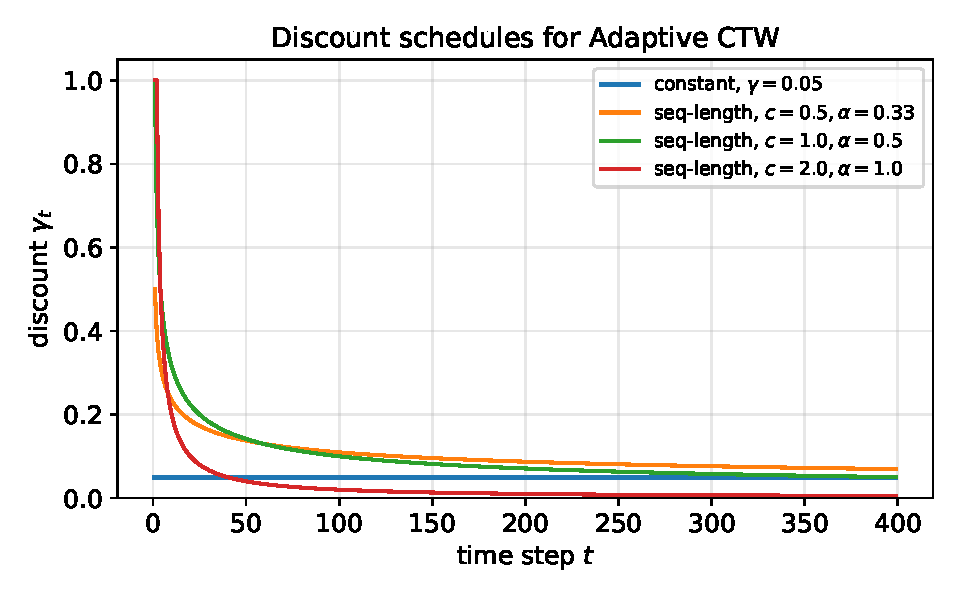
\includegraphics[width=0.6\textwidth]{discount_schedules}
  \end{center}
  \explain{The flat blue line is a constant discount $\gamma=0.05$. The
  curved lines are sequence-length discounts $\gamma_t=ct^{-\alpha}$ for
  different $(c,\alpha)$: early on (small $t$) they discount aggressively,
  then decay toward zero, converging to behavior close to the undiscounted
  KT estimator once enough data has accumulated. Larger $\alpha$ decays
  fastest.}
\end{frame}

\begin{frame}[fragile]{Python: Discounted vs. Standard KT Estimator}
  We compare standard vs.\ discounted ($\gamma=0.3$) KT estimators on an
  abrupt regime change, $x_{1:10}=0,0,0,0,0,1,1,1,1,1$, tracking the
  predicted probability of the \emph{next} symbol being a 1.
  \begin{lstlisting}[language=Python]
gamma = 0.3
seq = [0,0,0,0,0, 1,1,1,1,1]

a_std = b_std = 0.0          # standard KT counts
a_dis = b_dis = 0.0          # discounted KT counts
for x in seq:
    a_std += (x == 0); b_std += (x == 1)               # never decays
    if x == 0:
        a_dis = (1 - gamma) * (1 + a_dis); b_dis = (1 - gamma) * b_dis
    else:
        a_dis = (1 - gamma) * a_dis; b_dis = (1 - gamma) * (1 + b_dis)

pred_std = (b_std + 0.5) / (a_std + b_std + 1)   # P(x_11=1), standard KT
pred_dis = (b_dis + 0.5) / (a_dis + b_dis + 1)   # P(x_11=1), discounted KT
# pred_std = 0.5000   (a_std=5, b_std=5: perfectly "balanced," slow to react)
# pred_dis = 0.7471   (a_dis=0.326, b_dis=1.941: old 0-run mostly forgotten)
  \end{lstlisting}
  \explain{Standard KT ends up with $a_{std}=5,\,b_{std}=5$: it treats the
  five 0s and five 1s as equally important, giving a ``coin-flip''
  prediction of $0.5$, even though the \emph{most recent} five symbols were
  all 1s. Discounted KT shrinks $a_{dis}$ to about $0.33$ while $b_{dis}$
  grows to about $1.94$ (the 0-run gets discounted away), giving a far more
  responsive prediction of about $0.747$ that the next symbol is also 1.}
\end{frame}

% =============================================================================
\section{5.2 Context Tree Switching}
% =============================================================================

\begin{frame}[allowframebreaks]{Motivation: When the Model Class Itself Changes}
  The \textbf{Context Tree Switching (CTS)} algorithm [VNHB12] extends the
  CTW algorithm to a larger model class without losing much in terms of
  redundancy (extra bits needed compared to knowing the true model) or
  computation time. CTW works well provided the dynamics of the true
  environment \emph{never change}. This is a strong assumption, especially
  for tasks like data compression, where there might be an abrupt change in
  the data source partway through (e.g.\ the boundary between image data and
  text data within the same file).

  \bigskip
  \textbf{Example 5.2.1 (Piecewise 1-Markov source).} Consider the
  deterministic 0-Markov distribution $\mu_0(x_t=1\mid x_{<t})=1$ (always
  predicts 1) and the deterministic 1-Markov distribution
  $\mu_1(x_t=1\mid x_{<t})=\mu_1(1\mid x_{t-1})=1-x_{t-1}$ for $t>1$ and
  $\mu_1(x_1=0)=1$ (always \emph{flips} the previous bit). Now consider the
  alternating sequence
  \[
    \dot{x}_{1:\infty} = (01)^{100}(11)^{100}(01)^{100}(11)^{100}\cdots
  \]
  which is still deterministic, but now a \emph{non-stationary} 1-Markov
  process $\mu(x_t\mid x_{<t})=\mu_{i_t}(x_t\mid x_{<t})$ for
  $i_t := \lfloor (t+199)/200 \rfloor \bmod 2$.
  \explain{$\mu$ (mu) is the true, unknown data-generating distribution.
  $i_t$ just picks out which of the two rules ($\mu_0$ or $\mu_1$) is active
  at time $t$: it alternates every 200 symbols. The sequence is built from
  200-bit blocks: first $(01)^{100}$ (i.e.\ ``01'' repeated 100 times $=$ 200
  alternating bits), then $(11)^{100}$ (200 bits, all 1s), then the pattern
  repeats.}

  \framebreak

  Using a \emph{new} CTW tree (with $D=1$) every 200 time steps would work
  well on this sequence: the first and third blocks would learn the rule
  $0\to1,1\to0$ and the second and fourth would learn to always predict $1$
  regardless of context. However, we would expect a \emph{single} CTW model
  with $D=1$ for the \emph{entire} sequence to perform poorly: all the time
  spent collecting statistics in the first half of the sequence would
  actively \emph{hamper} learning in the second half.

  \medskip
  We can observe this via experiment: train four independent CTW models of
  depth 1, switching them out every 200 time steps, and compare against
  single CTW models of depth 1, 2, and 200 run over the whole sequence. Depth
  2 should be (almost) sufficient to learn the non-stationary sequence, since
  the rules $01\to0,\,10\to1,\,11\to1$ describe the sequence entirely, apart
  from the boundaries, where we briefly see the substrings $011$ and $110$
  (the process is nearly 2-Markov, more generally [VCH18]). Depth 200 can
  \emph{eventually} learn the boundary conditions too, but only given a much
  longer sequence than we use here.
\end{frame}

\begin{frame}[allowframebreaks]{Recreating Figure 5.1: Instantaneous KL Divergence}
  \begin{center}
    
\includegraphics[width=0.6\textwidth]{kl_divergence}
  \end{center}

  \framebreak

  \explain{We measure the \textbf{instantaneous KL divergence}
  $\mathrm{KL}(\mu\|\xi_{\CTW}) = -\ln\xi_{\CTW}(\dot x_t\mid \dot x_{<t})$
  (since $\mu$ is deterministic, only one sequence can ever occur, so the
  expectation in the general KL formula (Def.\ 4.2.11) collapses to this
  single term). $\xi$ (xi) denotes the model's predicted probability of the
  actual next bit. Dotted vertical lines mark the 200-bit block boundaries.

  \framebreak

  A single CTW model with $D=1$ spikes badly at every switch and, worse,
  performs poorly for the entire second occurrence of the $(11)^{100}$
  block (bits 400--600) because the statistics collected during the first
  half hamper it. $D=2$ handles the switches far better. $D=200$ needs to
  learn the boundary positions themselves and struggles more within each
  block early on. The \textbf{switch} model (four fresh $D=1$ CTW models,
  one per block) recovers a clean, low, repeating learning curve every
  time -- this is exactly the behavior CTS is designed to obtain
  automatically, without hardcoding the switch points.}
\end{frame}

\begin{frame}[allowframebreaks]{Towards CTS: the Switch Distribution}
  As previously discussed, the CTW mixture $\xi$ (xi) will eventually
  converge to the best single model in its class $\mathcal{M}$, but for CTW
  to guarantee the true environment is actually \emph{in} $\mathcal{M}$, we
  may need an extremely large choice of depth $D$ (and therefore many more
  bits from the environment before the parameters are well learned).

  \medskip
  Motivated by Example 5.2.1, we instead aim to find the \emph{best sequence
  of models} to learn the true environment, allowing for the possibility
  that the environment itself may change over time. This is the core idea
  behind CTS. What remains is to define a method, analogous to CTW, that can
  switch between models efficiently. First we need a distribution over
  \emph{sequences of models}.

  \framebreak

  \begin{block}{Definition 5.2.2 (Switch distribution [VNHB12])}
    \small
    Given a non-empty model class $\mathcal{M}=\{\rho_1,\rho_2,\dots,\rho_{|\mathcal{M}|}\}$,
    the \emph{switch distribution} with respect to $\mathcal{M}$ is defined
    as a weighted sum over all length-$n$ model-index sequences
    $i_{1:n}\in\{1,2,\dots,|\mathcal{M}|\}^n$:
    \[
      \tau_\alpha(x_{1:n}) := \sum_{i_{1:n}\in\{1,\dots,|\mathcal{M}|\}^n} w(i_{1:n})\prod_{k=1}^{n}\rho_{i_k}(x_k\mid x_{<k})
    \]
  \end{block}

  \framebreak

  \begin{block}{Definition 5.2.2, continued: the weight $w$}
    \small
    The weight $w$ is recursively defined as
    \[
      w(i_{1:n}) :=
      \begin{cases}
        1 & n=0\\
        \frac{1}{|\mathcal{M}|} & n=1\\
        w(i_{<n})\cdot(1-\alpha_n) & i_n=i_{n-1}\\
        w(i_{<n})\cdot\frac{\alpha_n}{|\mathcal{M}|-1} & i_n\ne i_{n-1}
      \end{cases}
    \]
    with switch rates $\alpha_n\in[0,1]$.
  \end{block}

  \framebreak

  \explain{$\rho_i$ (rho) is the $i$-th candidate model in a \emph{finite}
  model class $\mathcal{M}$ (a set of $|\mathcal{M}|$ predictors). $i_{1:n}$
  is a length-$n$ sequence choosing, at every time step, \emph{which} model
  is ``in charge''. $w(i_{1:n})$ is the prior probability of that particular
  sequence of model choices: switching to a \emph{different} model at step
  $n$ costs probability $\alpha_n/(|\mathcal{M}|-1)$ (split evenly among the
  other candidates), while \emph{staying} with the same model costs
  $1-\alpha_n$. $\alpha_n$ (alpha) is the switch rate at time $n$: the prior
  probability of switching to a new, uniformly-chosen model at that step.}
\end{frame}

\begin{frame}[fragile]{Algorithm 5.1: Efficiently Computing $\tau_\alpha$}
  Computing $\tau_\alpha$ naively is intractable: the sum ranges over
  $O(|\mathcal{M}|^n)$ sequences. It can, however, be computed in
  $O(n|\mathcal{M}|)$ time and $O(|\mathcal{M}|)$ space.
  \begin{block}{Algorithm 5.1 (Switch distribution $\tau_\alpha(x_{1:n})$)}
    \small
    \textbf{Require:} model class $\mathcal{M}=\{\rho_1,\dots,\rho_{|\mathcal{M}|}\}$;
    weights $w_i=1/|\mathcal{M}|$; switch rates $\alpha_2,\dots,\alpha_n$.\\
    \textbf{for} $t=1$ to $n$ \textbf{do}
    \begin{align*}
      \tau(x_t\mid x_{<t}) &:= \textstyle\sum_{i=1}^{|\mathcal{M}|} w_i\,\rho_i(x_t\mid x_{<t}) \\
      w_i &:= \frac{\alpha_{t+1}}{|\mathcal{M}|-1} + \Big((1-\alpha_{t+1})-\frac{\alpha_{t+1}}{|\mathcal{M}|-1}\Big)\frac{w_i\rho_i(x_t\mid x_{<t})}{\tau(x_t\mid x_{<t})}\quad\forall i
    \end{align*}
    \textbf{return} $\tau(x_{1:n})=\prod_{t=1}^n \tau(x_t\mid x_{<t})$
  \end{block}
  \explain{At each step, we first compute the mixture prediction
  $\tau(x_t|x_{<t})$ (a weighted vote of all models using their
  \emph{current} weights $w_i$), then update every weight $w_i$ using
  \emph{Bayes' rule combined with the switching prior} -- a model that
  predicted the observed symbol well gets a larger share of the posterior
  weight (the ratio $w_i\rho_i(x_t|x_{<t})/\tau(x_t|x_{<t})$), which is then
  blended with the fixed switch-prior probabilities $\alpha_{t+1}$ for next
  time step. This costs $O(|\mathcal{M}|)$ work per symbol.}
\end{frame}

\begin{frame}[fragile]{Python: Switch Distribution on a Toy 2-Model Class}
  Let $\mathcal{M}=\{\rho_1,\rho_2\}$ with $\rho_1=\mathrm{Bernoulli}(0.9)$
  (mostly predicts 1) and $\rho_2=\mathrm{Bernoulli}(0.1)$ (mostly predicts
  0), constant switch rate $\alpha=0.1$, and observed data
  $x_{1:6}=1,1,1,0,0,0$ (three 1s, then three 0s -- a regime switch at
  $t=4$).
  \begin{lstlisting}[language=Python]
rho1 = lambda x: 0.9 if x == 1 else 0.1     # model 1: "mostly ones"
rho2 = lambda x: 0.1 if x == 1 else 0.9     # model 2: "mostly zeros"
w = [0.5, 0.5]; alpha = 0.1
for x in [1, 1, 1, 0, 0, 0]:
    r = [rho1(x), rho2(x)]
    tau = w[0]*r[0] + w[1]*r[1]              # mixture prediction
    w = [alpha + (1 - 2*alpha) * (w[i]*r[i] / tau) for i in range(2)]
# t : tau(x_t|x_<t)   w1      w2
# 1 : 0.5000  ->  0.8200  0.1800
# 2 : 0.7560  ->  0.8810  0.1190
# 3 : 0.8048  ->  0.8882  0.1118
# 4 : 0.1895  ->  0.4750  0.5250   (regime switch: x_4 = 0 hurts model 1)
# 5 : 0.5200  ->  0.1731  0.8269
# 6 : 0.7615  ->  0.1182  0.8818   (switch model has now "found" model 2)
  \end{lstlisting}
  \explain{After the three 1s, weight has piled onto $\rho_1$
  ($w_1\approx0.888$). The moment 0s start arriving at $t=4$, $\rho_1$'s
  poor predictions ($\rho_1(0)=0.1$) cause its posterior weight to collapse,
  and by $t=6$ the switch distribution has shifted almost all its weight
  ($w_2\approx0.882$) onto $\rho_2$ -- exactly the behavior we want when the
  underlying source changes mid-sequence.}
\end{frame}

\begin{frame}[allowframebreaks]{From Switch Distribution to Context Tree Switching}
  \textbf{Context Tree Switching (CTS)} combines the switch distribution
  with CTW. Let $x_{1:n}^s$ denote the subsequence of $x_{1:n}$ of elements
  that follow the substring (context) $s$. For example, let
  $x=01011010$: the substring $01$ occurs starting at positions 1, 3, and 6,
  and the symbol immediately following each occurrence is $0$, $1$, and $0$
  respectively, giving $x^{01}=010$.
  \explain{$x^s_{1:n}$ formalizes ``the symbols that came right after we saw
  context $s$'' -- exactly the data used to update the KT counts at context
  node $s$ in a context tree.}

  \medskip
  Recall (\S4.5.2) that for a $k$-Markov environment with unknown
  $k\le D$, CTW chooses a mixture of all depth-$\le D$ PST (prediction
  suffix tree) models, weighted by complexity. The recursive definition of
  the probability $\mathrm{P}_w(s)$ associated with node $s$ is:
  \begin{block}{CTW mixture at node $s$}
  \[
    \mathrm{P}_w(s) :=
    \begin{cases}
      \tfrac12 \mathrm{P}_{\KT}(a_s,b_s) + \tfrac12 \mathrm{P}_w(0s)\mathrm{P}_w(1s) & \ell(s)<D\\
      \mathrm{P}_{\KT}(a_s,b_s) & \ell(s)=D
    \end{cases}
  \]
  \end{block}
  \explain{$\ell(s)$ (script-ell) is the length of context $s$. $0s$ and
  $1s$ denote the two child contexts obtained by extending $s$ with a
  further bit of history. This is a weighted average: half the weight goes
  to ``stop splitting here and just use the plain KT estimator at this
  node,'' and half goes to ``keep splitting into two finer sub-contexts.''
  CTS generalizes this by providing a weighted mixture over \emph{all
  sequences} of depth-$\le D$ PST models, allowing the best choice of model
  to change as the environment does.}
\end{frame}

\begin{frame}[allowframebreaks]{Definition 5.2.4: Context Tree Switching Probability}
  \begin{block}{Definition 5.2.4 (Context Tree Switching)}
    The Context Tree Switching probability $\mathrm{P}_{s,D}^{\CTS}$ of
    $x_{1:n}$, with depth $D>0$ and context $s$, is defined as
    \[
      \mathrm{P}_{s,D}^{\CTS}(x_{1:n})
      = \sum_{i_{1:n_s}\in\mathbb{B}^{n_s}} w(i_{1:n_s})
      \prod_{k=1}^{n_s}
      \begin{cases}
        \mathrm{P}_{\KT}\big((x^s_{1:n})_k \mid (x^s_{1:n})_{<k}\big) & i_k=0\\
        \mathrm{P}^{\CTS}_{0s,D-1}\big(x_{t_s(k)}\mid x_{<t_s(k)}\big)\,\mathrm{P}^{\CTS}_{1s,D-1}\big(x_{t_s(k)}\mid x_{<t_s(k)}\big) & i_k=1
      \end{cases}
    \]
    where $n_s=\ell(x^s_{1:n})$, $(x^s_{1:n})_{1:k}$ is the first $k$ bits of
    $x^s_{1:n}$, $t_s(k)=\min\{t\mid \ell(x^s_{1:t})=k\}$, and
    $\mathrm{P}_{s,D}^{\CTS}(y\mid x):=\mathrm{P}_{s,D}^{\CTS}(xy)/\mathrm{P}^{\CTS}_{s,D}(x)$.
    Base cases: $\mathrm{P}^{\CTS}_{s,0}(x_{1:n}):=\mathrm{P}_{\KT}(x^s_{1:n})$
    and $\mathrm{P}^{\CTS}_{s,D}(\epsilon)=1$. The top-level mixture
    $\mathrm{P}^{\CTS}_{\epsilon,D}(x_{1:n})$ is written $\mathrm{P}^{\CTS}_D(x_{1:n})$.
  \end{block}
  \explain{This is intentionally dense -- read it as: we take a weighted
  sum, over all binary ``choice sequences'' $i_{1:n_s}$ of length $n_s$
  (using the switch-distribution weight $w$ from Definition 5.2.2 applied to
  a 2-model class), where at each step the current symbol is generated
  \emph{either} by the plain KT estimator ($i_k=0$) \emph{or} recursively by
  the CTS mixture one level deeper in the tree ($i_k=1$). The product can be
  understood as an application of the chain rule, but on every step the
  \emph{sequence} $i_{1:n_s}$ dictates whether the KT estimator should be
  applied ($i_k=0$), or the recursive CTS mixture ($i_k=1$).}

  \framebreak

  \textbf{Computing $\mathrm{P}^{\CTS}_D$ efficiently.} CTS works much like
  the CTW method by using a perfect binary tree of depth $D$, where each
  node $s$ in the tree stores: $\mathrm{P}_{\KT}(a_s,b_s)$ (the base KT
  estimator associated with node $s$, along with the usual KT counts $a_s$
  and $b_s$); $\alpha_s$ and $\beta_s$ (beta), used like the switching
  weights $w$; and $\mathrm{P}^{\CTS}_s$, used like $\mathrm{P}_w$ in
  switching. Each internal node is initialized with
  $\alpha_s(\epsilon)=\beta_s(\epsilon)=\tfrac12$ and each leaf node with
  $\alpha_s(\epsilon)=1,\beta_s(\epsilon)=0$. When a new symbol $x_n$
  occurs, given a history $x_{<n}$, the path of the tree reflecting the
  context $x_{<n}$ is traversed and updated according to Algorithm 5.2.

  \medskip
  The update takes time $O(D)$ -- asymptotically the same as CTW -- and the
  space requirement asymptotically matches CTW too: it looks like $2^D$, but
  at most $O(n|D|)$ nodes need be created and stored explicitly (only nodes
  actually visited by the data get allocated).

  \medskip
  In the theorem to follow, we informally imagine $x_{1:n}$ as sampled from
  a \textbf{binary prediction suffix tree} $(\mathcal{S},\Theta_{\mathcal{S}})$,
  though the formal statement does not rely on this assumption and holds for
  all sequences $x_{1:n}$. $\mathcal{S}$ is a set of contexts belonging to
  class $\mathcal{C}_D$, and $\Theta_{\mathcal{S}}$ is a parameter vector
  associated with each context $s\in\mathcal{S}$: each parameter
  $\theta_s$ (theta) $\in[0,1]$ is the probability of observing a 1 given
  context $s$. The function $d(\mathcal{S})$ denotes the maximum length of
  any context $s\in\mathcal{S}$ (the complexity of the suffix tree model).
\end{frame}

\begin{frame}[allowframebreaks]{Algorithm 5.2: The CTS Update}
  \begin{block}{Algorithm 5.2 (Context Tree Switching update [VNHB12,BVT14])}
    \small
    \textbf{Require:} new symbol $x_n$; history $x_{<n}$; current context
    tree $\mathcal{T}_D=\{a_s,b_s,\alpha_s,\mathrm{P}^s_{\KT},\beta_s : s\in\mathbb{B}^D\}$.\\
    \textbf{for} $d=0$ to $D$ \textbf{do}
    \begin{itemize}\setlength\itemsep{0pt}
      \item[] Let $s=x_{n-d:n-1}$ be the current context.
      \item[] Update estimator $a_s,b_s$ and $\mathrm{P}^s_{\KT}$ with KT-updating; $x':=x_{n-\ell(s)-1}$.
      \item[] \textbf{if} $s$ is a leaf node \textbf{then}
        \[
          \alpha_s(x_{1:n}):=\alpha_s(x_{<n})\mathrm{P}^s_{\KT},\qquad
          \mathrm{P}^{\CTS}_{s,D}(x_{1:n}):=\alpha_s(x_{1:n})
        \]
      \item[] \textbf{else}
        \begin{align*}
          \mathrm{P}^{\CTS}_{s,D}(x_{1:n}) &:= \alpha_s(x_{<n})\mathrm{P}^s_{\KT} + \beta_s(x_{<n})\mathrm{P}^{\CTS}_{x's,D-1}(x_n\mid x_{<n})\\
          \alpha_s(x_{1:n}) &:= \tfrac{1}{n+1}\mathrm{P}^{\CTS}_{s,D}(x_{1:n}) + \tfrac{n-1}{n+1}\alpha_s(x_{<n})\mathrm{P}^s_{\KT}\\
          \beta_s(x_{1:n}) &:= \tfrac{1}{n+1}\mathrm{P}^{\CTS}_{s,D}(x_{1:n}) + \tfrac{n-1}{n+1}\beta_s(x_{<n})\mathrm{P}^{\CTS}_{x's,D-1}(x_n\mid x_{<n})
        \end{align*}
    \end{itemize}
  \end{block}
  \explain{This walks the context tree from the deepest relevant node
  ($d=0$, longest context) up to the root ($d=D$, shortest/no context),
  updating each node's KT counts and then blending ``stay with the plain KT
  model at this node'' ($\alpha_s$ weight) against ``switch to trusting one
  level deeper'' ($\beta_s$ weight), with the mix rate itself adapting over
  time via the $\tfrac{1}{n+1}$ / $\tfrac{n-1}{n+1}$ terms (mirroring
  Definition 5.2.2's switch rate, but self-tuning rather than a fixed
  $\alpha_n$).}
\end{frame}

\begin{frame}[allowframebreaks]{Theorem 5.2.5: PST-CTS Redundancy}
  \textbf{Redundancy} measures the gap between the optimal coding length
  (if the true model were known in advance) and the coding length actually
  achieved by a method -- lower redundancy means better compression /
  prediction performance.

  \begin{block}{Theorem 5.2.5 (PST-CTS redundancy [VNHB12])}
    Given a data sequence $x_{1:n}\in\mathbb{B}^n$ and PST
    $(\mathcal{S},\Theta_{\mathcal{S}})$ with $\mathcal{S}\in\mathcal{C}_D$
    and parameter vector $\Theta_{\mathcal{S}}:\{\theta_s\in[0,1]\}_{s\in\mathcal{S}}$,
    letting $d(\mathcal{S}):=\max_{s\in\mathcal{S}}\ell(s)$, the redundancy
    of the CTS coding distribution compared to coding with respect to the
    PST is upper bounded by
    \[
      \log_2\mathrm{P}_{\mathcal{S},\Theta_{\mathcal{S}}}(x_{1:n}) - \log_2\mathrm{P}^{\CTS}_D(x_{1:n})
      \;\le\; \Gamma_D(\mathcal{S}) + (d(\mathcal{S})+1)\log_2(n) + \frac{|\mathcal{S}|}{2}\log_2\!\Big(\frac{n}{|\mathcal{S}|}\Big) + |\mathcal{S}|
    \]
  \end{block}
  \explain{$\Gamma_D(\mathcal{S})$ (Gamma) is the model-cost complexity of
  the suffix set/tree $\mathcal{S}$ (essentially, the number of bits needed
  to describe the tree's shape, from Definition 4.3.20). $(d(\mathcal{S})+1)\log_2(n)$
  accounts for the maximum context length in the model together with the
  sequence length. $\tfrac{|\mathcal{S}|}{2}\log_2(n/|\mathcal{S}|)$ is the
  usual per-parameter estimation cost (trading off the number of contexts
  against the amount of data). $|\mathcal{S}|$ is simply the total number of
  contexts in the model. In words: CTS's redundancy is bounded by a
  combination of model complexity, maximum context length, and sequence
  length.}

  \framebreak

  \textbf{Comparing with CTW.} Recall the redundancy bound proven for the
  plain CTW method (Corollary 4.5.14):
  \[
    \log_2\mathrm{P}_{\mathcal{S},\Theta_{\mathcal{S}}}(x_{1:t}) - \log_2\mathrm{P}_D^{\CTW}(x_{1:n})
    \;\le\; \frac{|\mathcal{S}|}{2}\log_2\!\frac{n}{|\mathcal{S}|} + \Gamma_D(\mathcal{S}) + |\mathcal{S}|
  \]
  CTS has a slightly \emph{looser} redundancy bound, with one additional
  term $(d(\mathcal{S})+1)\log_2 n$ that grows only \emph{logarithmically}
  with the sequence length and \emph{linearly} with the depth of the PST
  modeling the true environment. This is a small penalty to pay in exchange
  for CTS having a much \emph{larger} model class -- one that allows
  switching between different Markov models in $\mathcal{C}_D$ over time --
  whereas plain CTW can, in a sense, only consider a single fixed model in
  $\mathcal{C}_D$ (the one most similar to the true environment) for the
  \emph{entire} sequence.
\end{frame}

% =============================================================================
\section{5.3 Partition Tree Weighting}
% =============================================================================

\begin{frame}{Motivation: Piecewise Stationary Sources}
  \textbf{Partition Tree Weighting (PTW)} [VWBG13] is an approach similar to
  Context Tree Weighting that is made for dealing with multiple, piecewise
  stationary data sources. A piecewise stationary data-generating source is
  defined by a partition \emph{over time} of several different data
  sources. As the name suggests, PTW uses a Bayesian mixture which weighs
  over \emph{choices of partitions} (rather than choices of contexts, as
  CTW does).

  \medskip
  Partition sources occur naturally in practice: for example, the weather
  follows a different distribution in summer than in winter. We can model
  this as a \textbf{temporal partition}, letting us essentially condition on
  time.

  \begin{block}{Definition 5.3.1 (Temporal partition)}
    A \emph{temporal partition} $\mathcal{P}_n\subseteq\mathbb{N}^+\times\mathbb{N}^+$
    is a set of tuples representing segments such that for all $x\in\mathbb{N}^+$
    with $x\le n$, there exists a unique $(a,b)\in\mathcal{P}_n$ with
    $a\le x\le b$. Each tuple is called a \emph{part}. We also define $f(x)$
    as the function that returns the index of the time segment containing $i$.
  \end{block}
  \explain{A temporal partition of $\{1,\dots,n\}$ is a partition into
  \emph{contiguous} blocks of time indices, e.g.\ $\mathcal{P}_{10}=
  \{(1,3),(4,6),(7,7),(8,10)\}$ corresponds to grouping time steps as
  $\{\{1,2,3\},\{4,5,6\},\{7\},\{8,9,10\}\}$: every subset must be a run of
  consecutive integers, unlike a general partition of a set.}
\end{frame}

\begin{frame}{Piecewise Stationary Sources}
  \begin{block}{Definition 5.3.2 (Piecewise (stationary) source)}
    We call $\rho$ a \emph{piecewise stationary source} if there exist
    probability measures $\{\rho_1,\rho_2,\dots\}$ and a partition
    $\mathcal{P}=\{(a_1,b_1),(a_2,b_2),\dots\}$ on $\mathbb{N}^+$ such that
    for all $n\in\mathbb{N}^+$ and all $x_{1:n}\in\mathbb{B}^n$,
    \[
      \rho(x_{1:n}) = \prod_{i\in\mathbb{N}^+} \rho_i(x_{a_i:b_i}).
    \]
  \end{block}
  \explain{The sequence is chopped into contiguous blocks by the partition
  $\mathcal{P}$, and within each block $i$ the data is generated stationarily
  by its own model $\rho_i$ (rho). We make no assumption that the true
  source $\mu$ actually has this form, but PTW is designed to predict/compress
  well \emph{when} $\mu$ looks like this (or piecewise i.i.d.).}

  \medskip
  With this we construct our model class: the set of \textbf{binary temporal
  partitions} $\mathcal{B}_D$. Imagine a complete binary tree of depth $D$
  with leaves numbered $1,\dots,2^D$. For a fixed suffix set/tree
  $\mathcal{S}\in\mathcal{C}_D$, associate each leaf $s\in\mathcal{S}$ with
  the interval spanned by the $2^{D-\ell(s)}$ leaves at level $D$, if we
  were to expand $s$ down to level $D$. The partition $\mathcal{P}$
  associated with $\mathcal{S}$ is the union of those intervals, and
  $\mathcal{B}_D$ is the set of \emph{all} such partitions.
\end{frame}

\begin{frame}{Binary Temporal Partitions, Illustrated}
  \begin{center}
    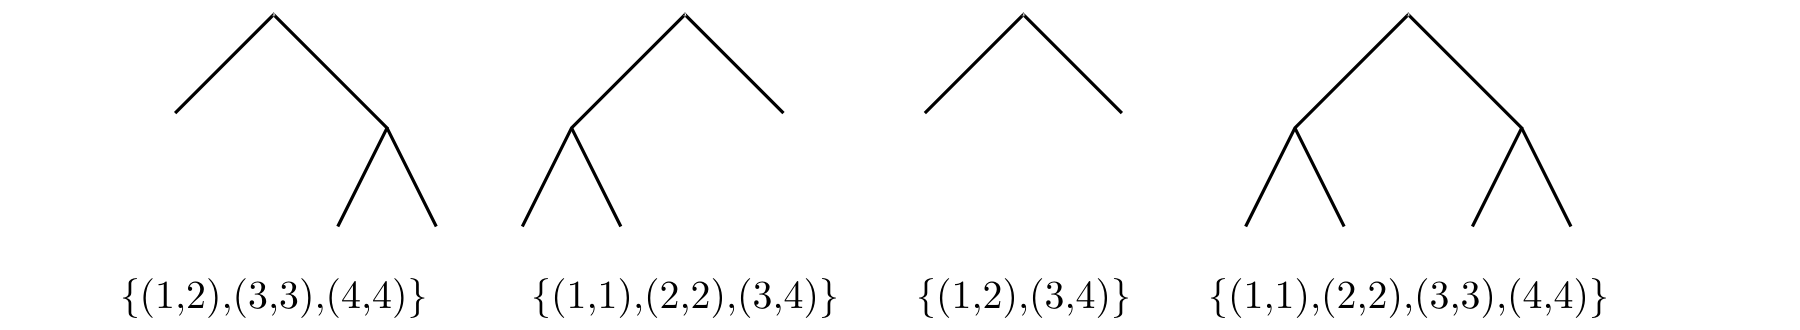
\includegraphics[width=0.85\textwidth]{partition_trees_b2}
  \end{center}
  \explain{Figure 5.2: all binary partitions of $\{1,2,3,4\}$ in
  $\mathcal{B}_2$, except the empty (root-only) tree giving $\{(1,4)\}$.
  Each tree shape corresponds to exactly one temporal partition. Note that
  e.g.\ $\{(1,3),(4,4)\}$ is \emph{not} in $\mathcal{B}_2$, since a
  length-3 part cannot arise from cutting a depth-2 binary tree cleanly.}
\end{frame}

\begin{frame}[allowframebreaks]{The Set $\mathcal{B}_D$, Two Ways}
  \begin{block}{Definition 5.3.3 (Set of all binary temporal partitions $\mathcal{B}_D$)}
    \[
      \mathcal{B}_D = \{\mathcal{P}(\mathcal{S}) : \mathcal{S}\in\mathcal{C}_D\}, \qquad
      \mathcal{P}(\mathcal{S}) := \{I_s : s\in\mathcal{S}\}
    \]
    \[
      I_s := \big(2^{D-\ell(s)}b(\mathrm{reverse}(s))+1,\; 2^{D-\ell(s)}(b(\mathrm{reverse}(s))+1)\big)
    \]
    where $b(\mathrm{reverse}(s))=\sum_{i=1}^{\ell(s)} 2^{i-1}s_i$ interprets
    the reversed bit string $s$ as a natural number (Proposition 2.1.1).
  \end{block}
  \explain{$b(\cdot)$ converts a bit string into the integer it represents,
  and $I_s$ computes exactly which contiguous block of the $2^D$ finest
  leaves corresponds to context node $s$. This is a direct (if fiddly)
  formula; the recursive definition below is more intuitive.}

  \begin{block}{Definition 5.3.4 (Set of all binary temporal partitions
  $\mathcal{B}_D$, recursively)}
    \[
      \mathcal{B}_0 := \{\{(1,1)\}\}, \qquad
      \mathcal{B}_{d+1} := \{\{(1,2^{d+1})\}\} \cup \{\mathcal{P}\cup(\mathcal{P}'+2^d) : \mathcal{P},\mathcal{P}'\in\mathcal{B}_d\}
    \]
    where $\mathcal{P}'+a$ shifts every interval in $\mathcal{P}'$ by $a$.
  \end{block}
  \explain{Base case: at depth 0 there is only one possible partition, the
  single point $\{(1,1)\}$. Recursive case: a valid depth-$(d{+}1)$
  partition of $\{1,\dots,2^{d+1}\}$ is \emph{either} the trivial
  ``no split at all'' partition $\{(1,2^{d+1})\}$, \emph{or} obtained by
  taking any valid depth-$d$ partition of the left half and any valid
  depth-$d$ partition of the right half (shifted over) and joining them.
  Proving Definitions 5.3.3 and 5.3.4 agree is left as Exercise 5.6.2.}
\end{frame}

\begin{frame}[allowframebreaks]{Definition 5.3.5 and Theorem 5.3.6: The PTW Probability}
  We now define the PTW method and the priors used for weighting. Like CTW
  we mix over a set of trees, but instead of mixing over \emph{all
  partitions} (choices of context split), we mix over binary temporal
  partitions $\mathcal{B}_D$, allowing us to easily define a measure of
  complexity based on the corresponding partition tree, using the same
  penalty as the CTW model cost (Definition 4.3.20). The base model $\rho$
  is left unspecified for now; possible choices include the KT estimator or
  even CTW itself.

  \begin{block}{Definition 5.3.5 (Partition Tree Weighting (PTW))}
    Let $\rho$ be some base model (such as the KT estimator). The
    \emph{Partition Tree Weighting probability} $\mathrm{P}_D^{\PTW}$ of
    string $x_{1:n}$ with depth $D$ is defined as
    \[
      \mathrm{P}_D^{\PTW}(x_{1:n}) := \sum_{\mathcal{P}\in\mathcal{B}_D} 2^{-\Gamma_D(\mathcal{P})}\prod_{(a,b)\in\mathcal{P}} \rho(x_{a:b})
    \]
    where $\Gamma_D(\mathcal{P}):=\Gamma_D(\mathcal{S}(\mathcal{P}))$ is the
    number of nodes in the partition tree $\mathcal{S}$ associated with
    $\mathcal{P}$ that have depth less than $D$.
  \end{block}
  \explain{This is a weighted average, over every possible way of chopping
  $x_{1:n}$ into a binary-temporal-partition-compatible set of blocks, of
  the product of the base model's probability on each block -- weighted by
  $2^{-\Gamma_D(\mathcal{P})}$, a prior that penalizes partitions with more
  ``splits'' (more internal nodes), in the same MDL spirit as CTW's model
  cost.}

  \framebreak

  Computing $\mathrm{P}_D^{\PTW}$ naively would take $O(2^{2^D})$ time (one
  term per partition, and there are that many trees of depth $D$). PTW
  admits a recurrence relation analogous to CTW's (4.5.2):
  \begin{block}{Theorem 5.3.6 (Recursive definition of PTW probability)}
    For any depth $D$ and sequence $x_{1:n}$ with $n\le 2^D$,
    \[
      \mathrm{P}_D^{\PTW}(x_{1:n}) = \tfrac12\rho(x_{1:n}) + \tfrac12\, \mathrm{P}_{D-1}^{\PTW}(x_{1:k})\,\mathrm{P}_{D-1}^{\PTW}(x_{k+1:n}), \qquad k=2^{D-1}.
    \]
  \end{block}
  \explain{Just like CTW's recursion mixes ``stop splitting the context''
  against ``split into two child contexts,'' PTW's recursion mixes ``treat
  the whole block $x_{1:n}$ as one stationary segment'' (weight $\tfrac12$,
  using the base model directly) against ``split time exactly in half and
  recurse on each half independently'' (weight $\tfrac12$). The proof
  follows the same pattern as Theorem 4.5.8.}
\end{frame}

\begin{frame}{PTW's Recursive Halving, Visualized}
  \begin{center}
    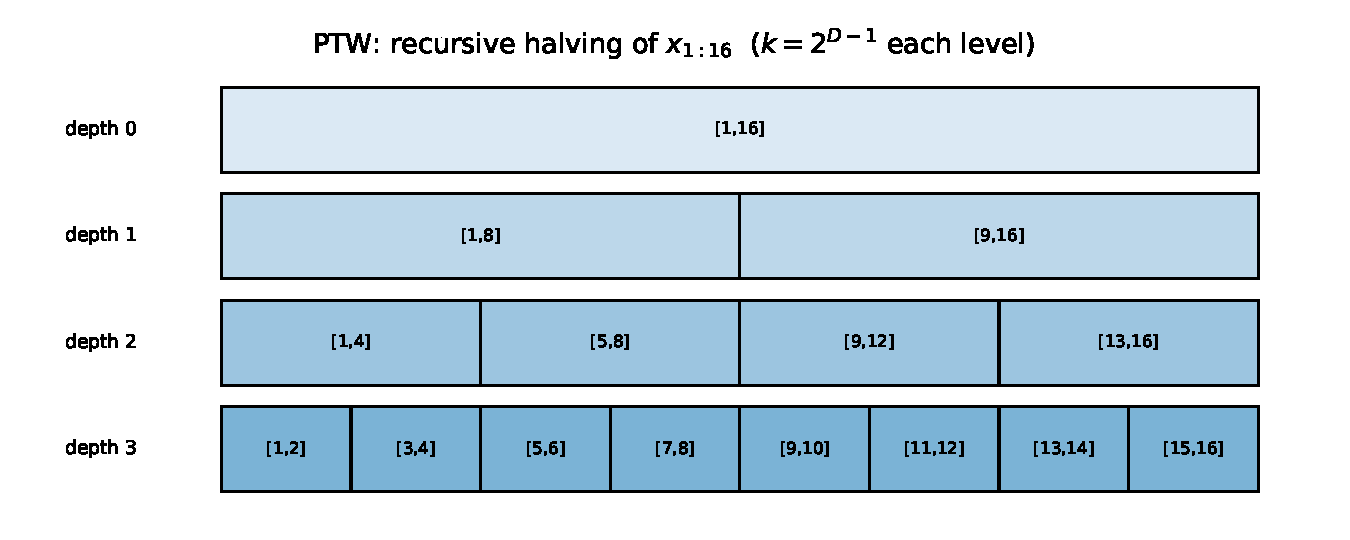
\includegraphics[width=0.85\textwidth]{ptw_recursion}
  \end{center}
  \explain{Each row is one level of recursion in Theorem 5.3.6: the interval
  $[1,16]$ (depth 0) either stays whole, or is split exactly in half at
  depth 1 into $[1,8]$ and $[9,16]$, and so on down to depth 3, where every
  block has length 2. PTW mixes over \emph{all} the ways of choosing, at
  every node, whether to stop splitting (``treat this block as one
  stationary chunk'') or to continue splitting -- exactly the binary
  temporal partitions of Definition 5.3.3/5.3.4.}
\end{frame}

\begin{frame}[allowframebreaks]{Algorithm 5.3: Computing PTW in $O(D)$ Space}
  Using Theorem 5.3.6, PTW can be computed recursively in $O(nD)$ time and
  $O(nD)$ space (storing the context tree in memory). The following
  algorithm improves this to $O(D)$ memory -- a critical improvement, since
  many choices of base model $\rho$ are themselves memory-intensive -- by
  exploiting the regular access pattern of the data structure. It works
  incrementally, one bit at a time; for each bit the context tree is
  traversed depth-first, then iterated back up to update the weights.

  \begin{block}{Algorithm 5.3 (Partition Tree Weighting $\mathrm{P}_D^{\PTW}(x_{1:n})$ [VWBG13])}
    \small
    \textbf{Require:} depth $D$; base model $\rho$. \textbf{Input:} data
    $x_{1:n}$, $n\le 2^D$.\\
    \textbf{for} $0\le j\le D$: $b_j:=1,\,w_j:=1,\,r_j:=1$\\
    \textbf{for} $t=1$ to $n$ \textbf{do}
    \begin{itemize}\setlength\itemsep{0pt}
      \item[] $i:=\mathrm{MSCB}_D(t)$
      \item[] $b_i:=w_{i+1}$
      \item[] \textbf{for} $j=i+1$ to $D$: $r_j:=t$
      \item[] $w_D:=\rho(x_{r_D:t})$
      \item[] \textbf{for} $i=D-1$ downto $0$: $w_i:=\tfrac12\rho(x_{r_i:t})+\tfrac12 w_{i+1}b_i$
    \end{itemize}
    \textbf{return} $w_0$
  \end{block}
  \explain{$\mathrm{MSCB}_D(t)$ (``most significant changed context bit'')
  is the index $i$ where the $D$-bit binary representations of $t-1$ and
  $t-2$ first differ (with $\mathrm{MSCB}_D(1):=0$). For example, at $d=5$,
  to compute $\mathrm{MSCB}_5(7)$ we compare the binary representation of 6
  ($00110$) and 5 ($00101$): they differ at index 3, so
  $\mathrm{MSCB}_5(7)=3$. Intuitively, this tells the algorithm exactly how
  far back up the tree it needs to ``close off'' a finished block and start
  a fresh one, without ever needing to store the whole tree.

  \framebreak

  The algorithm can be modified to run incrementally, computing
  $\mathrm{P}_D^{\PTW}(x_{1:n})$ given $\mathrm{P}_D^{\PTW}(x_{<n})$ in
  $O(D)$ time by only running the inner loop. One downside of PTW is that
  the depth $D$ must satisfy $n\le 2^D$ by the definition of a binary
  temporal partition. To make the running time as fast as possible, we
  choose $D=\lceil\log_2(n)\rceil$, giving $O(n\log n)$ time and
  $O(\log n)$ space overall.}
\end{frame}

\begin{frame}[fragile]{Python: PTW Probability by Hand ($D=2$, $n=4$)}
  Base model $\rho=$ KT estimator (i.i.d.\ assumption); $x_{1:4}=0,1,1,0$.
  We compute $\mathrm{P}_2^{\PTW}(x_{1:4})$ via Theorem 5.3.6's recursion.
  \begin{lstlisting}[language=Python]
import math
def PKT(bits):                              # KT probability of a bit-string
    a, b = bits.count(0), bits.count(1)
    num = 1.0
    for i in range(a): num *= (i + 0.5)
    for j in range(b): num *= (j + 0.5)
    return num / math.factorial(a + b)

x = [0, 1, 1, 0]
P0 = [PKT([b]) for b in x]                          # depth-0: single symbols
P1_12 = 0.5*PKT(x[0:2]) + 0.5*P0[0]*P0[1]            # depth-1, block [1,2]
P1_34 = 0.5*PKT(x[2:4]) + 0.5*P0[2]*P0[3]            # depth-1, block [3,4]
P2 = 0.5*PKT(x) + 0.5*P1_12*P1_34                    # depth-2, block [1,4]
# rho(0110) = 0.023438
# P1(01) = P1(10) = 0.1875
# P2(0110) = 0.5*0.023438 + 0.5*0.1875*0.1875 = 0.029297
  \end{lstlisting}
  \explain{The final mixture probability $0.029297$ blends "treat all four
  bits as one stationary block" (weight $\tfrac12$, using
  $\rho(0110)=0.0234$) against "split into two length-2 blocks and multiply
  their probabilities" (weight $\tfrac12$, using $0.1875\times0.1875$).
  Since $0.1875\times0.1875=0.03516$ is bigger than $\rho(0110)=0.0234$, the
  split hypothesis contributes the larger share, reflecting that treating
  $01$ and $10$ as two separate KT-fitted blocks explains this particular
  string slightly better than fitting one KT model to all four bits.}
\end{frame}

\begin{frame}[allowframebreaks]{Theorem 5.3.8 and 5.3.9: PTW Redundancy}
  \begin{block}{Theorem 5.3.8 (Upper bound on log PTW probability)}
    For all $n\in\mathbb{N}_0$, let $D=\lceil\log(n)\rceil$. Then for all
    $x_{1:n}$ and for all $\mathcal{P}\in\mathcal{B}_D$,
    \[
      -\log \mathrm{P}_D^{\PTW}(x_{1:n}) \;\le\; \Gamma_D(\mathcal{P}) - \sum_{(a,b)\in\mathcal{P}}\log(\rho(x_{a:b}))
    \]
  \end{block}
  \explain{This says: no matter which partition $\mathcal{P}$ you had in
  mind as ``the true one,'' PTW's coding cost is never worse than the cost
  of coding with exactly that partition, plus the $\Gamma_D(\mathcal{P})$
  bits needed to describe the partition's shape. Proof: drop every other
  term from the defining sum in Definition 5.3.5 (all terms are
  non-negative), leaving just the $\mathcal{P}$ term, then take $-\log$.}

  \framebreak

  \begin{block}{Theorem 5.3.9 (PTW redundancy)}
    Let $\mu$ be a piecewise stationary data-generating source and let the
    base model $\rho$ have redundancy with respect to a class $\mathcal{G}$
    of bounded-memory data-generating sources upper bounded by a
    non-negative, monotonically non-decreasing concave function
    $g:\mathbb{N}_0\to\mathbb{R}$ with $g(0)=0$. For all $n\in\mathbb{N}_0$,
    set $D=\lceil\log(n)\rceil$. There exists a constant $c$ such that the
    redundancy of PTW is upper bounded by
    \[
      \log\mu(x_{1:n}) - \log\mathrm{P}_D^{\PTW}(x_{1:n})
      \;\le\; \Big(2+g\Big(\Big\lceil\frac{n}{|\mathcal{P}|(D+1)}\Big\rceil\Big)\Big)|\mathcal{P}|(D+1)
    \]
  \end{block}
  \explain{$g$ (a stand-in for ``how good the base model $\rho$ is'')
  bounds the redundancy the base model would incur \emph{on its own}, per
  block. The theorem says PTW's overall redundancy stays controlled by that
  same function $g$, evaluated at roughly $n/|\mathcal{P}|$ (the typical
  block length), multiplied by the number of blocks and the tree depth. The
  proof (see the book) uses a refinement argument: any partition
  $\mathcal{P}$ can be approximated from within $\mathcal{B}_D$ by a
  slightly finer partition with at most $|\mathcal{P}|(D+1)$ segments, then
  applies Theorem 5.3.8 together with Jensen's inequality (since $g$ is
  concave).}

  \medskip
  \textbf{Takeaway.} PTW is a computationally efficient algorithm with
  strong theoretical guarantees whenever the truth is (close to) a piecewise
  stationary data-generating source.
\end{frame}

% =============================================================================
\section{5.4 Forget-Me-Not Process}
% =============================================================================

\begin{frame}[allowframebreaks]{The Forget-Me-Not (FMN) Process}
  \emph{(This explanation follows [WSB$^+$20, Sec.\ 4].)} Generalizing
  stationary algorithms to non-stationary environments is a key challenge in
  \textbf{continual learning}. The \textbf{Forget-Me-Not (FMN)} process is a
  probabilistic meta-algorithm tailored towards non-i.i.d., piecewise
  stationary, \emph{repeating} sources. This meta-algorithm takes as input a
  single base measure $\rho$ on target strings and \emph{extends} the
  Partition Tree Weighting algorithm to incorporate a memory of up to $k$
  previous model states in a data structure known as a \textbf{model pool}.
  It efficiently applies Bayesian model averaging over a set of
  \emph{postulated segmentations} of time (task boundaries) and a growing
  set $\mathcal{M}$ of stored base-model states $\rho(\cdot\mid s)$ for some
  subsequences of $x_{1:n}$, while providing a mechanism to either learn a
  new local solution or adapt/recall a previously learned one.

  \framebreak

  \begin{center}
    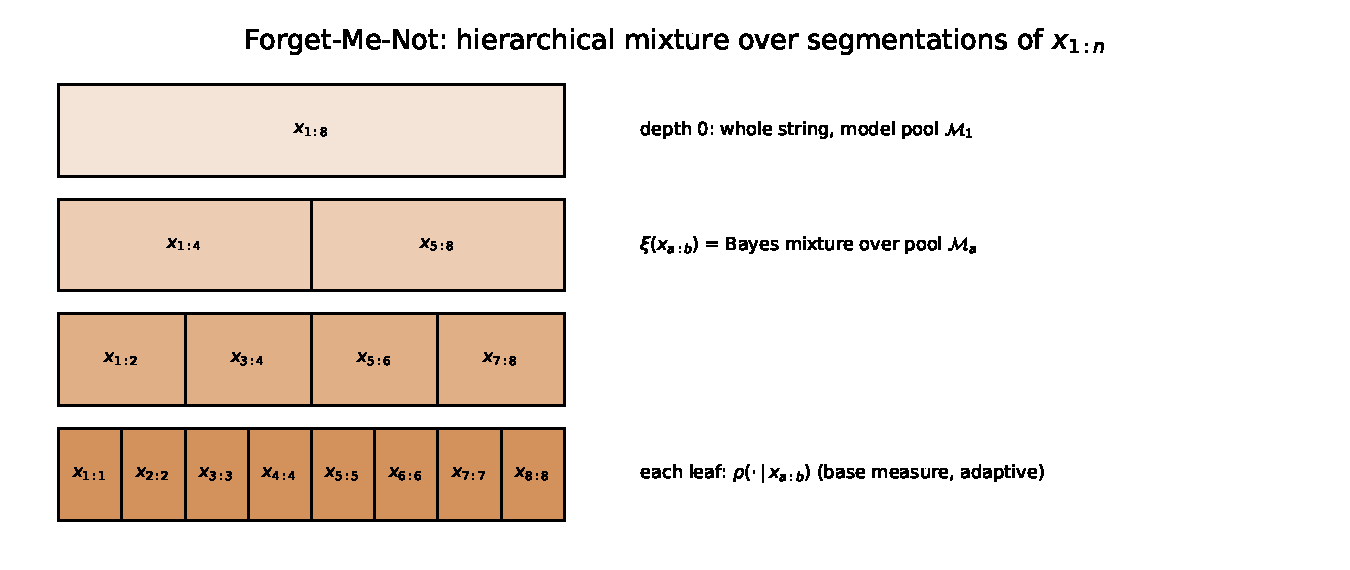
\includegraphics[width=0.85\textwidth]{fmn_pool}
  \end{center}
  \explain{FMN is derived and described in [MVK$^+$16]. It computes the
  probability $p'=\FMN_d(x_{1:n})\in[0,1]$ of a string of binary targets
  $x_{1:n}\in\{0,1\}^n$ of length $n$ -- e.g.\ $x_t$ could be a binary class
  label. It hierarchically Bayes-mixes an exponentially large,
  self-generated class of models from a base measure $\rho$ in
  $O(kn\log n)$ time and $O(k\log n)$ space, roughly as follows: for
  $n=2^d$, and for $j=0,\dots,d$, it breaks up $x_{1:n}$ into $2^j$ strings
  each of length $2^{d-j}$, exactly the recursive halving structure of PTW
  pictured above (compare to the PTW figure). For each substring $x_{a:b}$,
  associated to each node of the tree, we get a probability $\xi(x_{a:b})$
  obtained from a Bayesian mixture of \emph{all} models in the model pool
  $\mathcal{M}_a$ at time $a$. Taking any (variable-depth) subtree -- which
  induces a particular segmentation of time -- concatenating the strings at
  its leaves gives back $x_{1:n}$, so the product of their associated
  mixture probabilities gives a probability for $x_{1:n}$. Doing this and
  averaging over all $O(2^n)$ possible subtrees (which can be done
  incrementally, see [MVK$^+$16]) gives $\FMN_d(x_{1:n}\mid\rho)$ in
  $O(k\log n)$ time per string element.}

  \framebreak

  \textbf{The model pool.} The models in the model pool are generated from
  an arbitrary adaptive base measure $\rho$. For example, $\rho$ could be a
  Beta-Bernoulli model whose weights are updated using Bayesian inference,
  or something more sophisticated. At time $t$, $\mathcal{M}_t$ contains at
  most $k$ ``versions'' of $\rho$, with $\mathcal{M}_1:=\rho$. For
  $t=2,\dots,n$, whenever a string $x_{a:b}$ with $b=t$ is encountered, the
  model $\rho^*\in\mathcal{M}_a$ assigning the highest probability to the
  node's string $x_{a:b}$ is either \emph{added} to the model pool, i.e.\
  $\mathcal{M}_{t+1}=\mathcal{M}_t\cup\{\rho^*(\cdot\mid x_{a:b})\}$, or
  \emph{ignored} based on a Bayesian hypothesis test criterion given in
  [MVK$^+$16].
  \explain{Intuitively: whenever FMN encounters a block of data that looks
  like one it has seen before, it can \emph{recall} and reuse the matching
  stored model rather than relearning it from scratch -- this is the
  ``forget-me-not'' behavior that distinguishes FMN from plain PTW, which
  always starts a fresh model for every new segment.}
\end{frame}

% =============================================================================
\section{5.5 Context Tree Maximization}
% =============================================================================

\begin{frame}[allowframebreaks]{Context Tree Maximization (CTM)}
  Instead of a Bayesian \emph{mixture} over all prediction suffix trees, as
  CTW does, \textbf{Context Tree Maximization} selects the \textbf{Maximum A
  Posteriori (MAP)} tree (the symbolic index $\mathrm{m}$ stands for
  ``maximum''):
  \[
    \mathrm{P}_{\mathrm{m}}^D(x_{1:n}) = \max_{\mathcal{S}\in\mathcal{C}_D}\Big\{2^{-\Gamma_D(\mathcal{S})}\mathrm{P}_{\mathcal{S},\KT}(x_{1:n})\Big\}
  \]
  which is identical to Theorem 4.5.11, just with the \emph{sum} replaced by
  a \emph{max}. (Here $\mathrm{m}$ is not a variable, but a name for the
  maximizing probability.)
  \explain{Rather than averaging the probability every possible context
  tree $\mathcal{S}\in\mathcal{C}_D$ assigns to the data (weighted by its
  prior $2^{-\Gamma_D(\mathcal{S})}$), CTM simply asks: which \emph{single}
  tree $\mathcal{S}$ gives the largest (prior-weighted) probability?}

  \medskip
  Taking $-\log$ of both sides,
  $\min_{\mathcal{S}}\{-\log\mathrm{P}_{\mathcal{S},\KT}(x_{1:n})+\Gamma_D(\mathcal{S})\}$,
  we can interpret this as an application of the \textbf{Minimum
  Description Length (MDL)} principle (Definition 2.7.24): find the tree
  that minimizes (data coding cost) $+$ (model description cost).

  \framebreak

  Computing this maximum naively would need $O(2^{2^D})$ time (one term per
  tree). As with CTW, there is an efficient method, called \textbf{Context
  Tree Maximization} [WTS00,NSH12], computing this in $O(nD)$ time via the
  recurrence relation
  \[
    \mathrm{P}^D_{\mathrm{m},s}(x_{1:n}) :=
    \begin{cases}
      \tfrac12\max\{\mathrm{P}_{\KT}(a_s,b_s),\ \mathrm{P}^D_{\mathrm{m},0s}(x_{1:n})\mathrm{P}^D_{\mathrm{m},1s}(x_{1:n})\} & \ell(s)<D\\
      \mathrm{P}_{\KT}(a_s,b_s) & \ell(s)=D
    \end{cases}
  \]
  \explain{This mirrors CTW's recurrence exactly, but with the average
  $\tfrac12(\cdot)+\tfrac12(\cdot)$ replaced by $\tfrac12\max(\cdot,\cdot)$:
  at every node, keep whichever of ``stop here'' or ``split further'' gives
  the higher (weighted) probability.}
\end{frame}

\begin{frame}[allowframebreaks]{The Maximizing Tree and Theorem 5.5.1}
  Alongside the maximizing probability, we can also recursively track the
  \emph{maximizing suffix set} (i.e.\ which tree actually achieved the max):
  \[
    \mathcal{S}^D_{\mathrm{m},s}(x_{1:n}) :=
    \begin{cases}
      \mathcal{S}^D_{\mathrm{m},0s}(x_{1:n})\times\{0\}\ \cup\ \mathcal{S}^D_{\mathrm{m},1s}(x_{1:n})\times\{1\} & \parbox{5.2cm}{\raggedright if $\mathrm{P}_{\KT}(a_s,b_s) < \mathrm{P}^D_{\mathrm{m},0s}\mathrm{P}^D_{\mathrm{m},1s}$ and $\ell(s)<D$}\\[4pt]
      \{\epsilon\} & \text{otherwise}
    \end{cases}
  \]
  \explain{At each node, if splitting gave the strictly larger value, the
  maximizing tree below $s$ is the union of the two children's maximizing
  sub-trees (each extended by the bit that leads to it); otherwise, the
  maximizing tree here is just the trivial single-node tree $\{\epsilon\}$
  (stop splitting).}

  \begin{block}{Theorem 5.5.1 (Context Tree Maximization)}
    For any sequence $x_{1:n}\in\mathbb{B}^n$,
    \[
      \mathrm{P}^D_{\mathrm{m},\epsilon}(x_{1:n}) = \max_{\mathcal{S}\in\mathcal{C}_D}\{2^{-\Gamma_D(\mathcal{S})}\mathrm{P}_{\mathcal{S},\KT}(x_{1:n})\}, \qquad
      \mathcal{S}^D_{\mathrm{m},\epsilon}(x_{1:n}) = \operatorname*{arg\,max}_{\mathcal{S}\in\mathcal{C}_D}\{2^{-\Gamma_D(\mathcal{S})}\mathrm{P}_{\mathcal{S},\KT}(x_{1:n})\}
    \]
  \end{block}
  \explain{The recursively computed root values $\mathrm{P}^D_{\mathrm{m},\epsilon}$
  and $\mathcal{S}^D_{\mathrm{m},\epsilon}$ are exactly the MAP probability
  and MAP tree defined at the top of this section -- proving this (Exercise
  5.6.4) is a straightforward induction on the recurrence, exactly parallel
  to the proof that CTW's recurrence computes the true mixture (Theorem
  4.5.8).}
\end{frame}

\begin{frame}[fragile]{Python: CTM vs.\ CTW on a Small Example ($D=1$)}
  Take a sequence with counts $a_\epsilon=4,\,b_\epsilon=2$ at the root
  (context-free counts over the whole sequence), and, splitting by the
  preceding bit, $a_0=2,\,b_0=2$ (context ``previous bit was 0'') and
  $a_1=1,\,b_1=0$ (context ``previous bit was 1'') -- consistent with the
  actual sequence $x_{1:6}=0,0,0,1,0,1$.
  \begin{lstlisting}[language=Python]
import math
def PKT(a, b):
    num = 1.0
    for i in range(a): num *= (i + 0.5)
    for j in range(b): num *= (j + 0.5)
    return num / math.factorial(a + b)

P_root  = PKT(4, 2)              # "don't split": one KT model for everything
P_split = PKT(2, 2) * PKT(1, 0)  # "split": separate KT models per context
Pw_CTW  = 0.5*P_root + 0.5*P_split          # CTW: average the two
Pm_CTM  = max(P_root, P_split)              # CTM: keep the larger one
# P_root  = PKT(4,2) = 0.0068359     ("stay at the root")
# P_split = PKT(2,2)*PKT(1,0) = 0.0234375*0.5 = 0.0117188   ("split")
# Pw_CTW  = 0.0092773                (Bayesian mixture of both)
# Pm_CTM  = 0.0117188  ==  P_split   (CTM picks the SPLIT tree)
  \end{lstlisting}
  \explain{Since $P_{\text{split}}=0.011719$ is larger than
  $P_{\text{root}}=0.006836$, CTM's maximizing suffix set is the full
  depth-1 tree $\mathcal{S}=\{0,1\}$ (splitting on the previous bit) --
  correctly detecting that the next-bit distribution really does depend on
  the previous bit in this data. CTW's mixture $0.009277$ sits, as expected,
  between the two candidate values, since it hedges its bets over both
  trees rather than committing to one.}
\end{frame}

% =============================================================================
\section{5.6 Exercises}
% =============================================================================

\begin{frame}[allowframebreaks]{Exercises}
  \begin{enumerate}
    \item[\textbf{[C10]}] Show that the construction in Definition 5.3.3 is
      a bijection between $\mathcal{C}_D$ and $\mathcal{B}_D$. Convert the
      recursive definition of $\mathcal{C}_D$ to a direct recursive
      definition of $\mathcal{B}_D$. Show that $2^{-\Gamma_D(\mathcal{P})}$
      is a valid prior, i.e.\ prove that
      $\sum_{\mathcal{P}\in\mathcal{C}_D}\Gamma_D(\mathcal{P})=1$ for all
      $D\in\mathbb{N}_0$.
    \item[\textbf{[C15]}] Prove that the sets of all binary temporal
      partitions $\mathcal{B}_D$ defined in Definition 5.3.3 and Definition
      5.3.4 are indeed the same.
    \item[\textbf{[C25]}] Prove Theorem 5.3.6.
    \item[\textbf{[C20]}] Prove Theorem 5.5.1.
    \item[\textbf{[C30i]}] While the Krichevsky--Trofimov (KT) estimator is
      commonly used as a base model, the Context Tree Weighting (CTW)
      variants can operate with \emph{any} base model. Implement a
      selection of the variants in this chapter (Adaptive CTW, PTW, CTS,
      FMN, and CTM), using other variants (or even CTW itself) as the base
      model. Analyze their performance relative to using the KT estimator
      as the base model and identify which combinations yield the best
      results.
    \item[\textbf{[C35]}] Based on the combinations used in the previous
      exercise, deduce new redundancy bounds specifically tailored to these
      combinations.
    \item[\textbf{[C20]}] Explain why we cannot indefinitely chain
      predictors as base models. For instance, CTS with a PTW base model,
      further supported by a CTW base model, and another CTS base model,
      and so forth.
    \item[\textbf{[C30]}] From the previous exercise, validate your
      statement with a theoretical analysis of the gains/losses incurred
      each time this chaining process is executed. Further corroborate this
      claim with practical demonstrations by conducting experiments with
      this chaining procedure.
    \item[\textbf{[C35]}] Formulate a multi-alphabet version of Adaptive
      CTW, PTW, CTS, FMN, and CTM. Hint: use Section 4.6 and [PS99] as
      guiding references.
  \end{enumerate}
  \explain{The bracketed codes (e.g.\ [C10], [C30i]) are the book's standard
  difficulty/type ratings: the number is a rough difficulty score, ``C''
  marks a more conceptual/proof-based exercise, and ``i'' marks an
  implementation exercise.}
\end{frame}

% =============================================================================
\section{5.7 History and References}
% =============================================================================

\begin{frame}{History and References}
  See Section 4.7 (the history and references for Context Tree Weighting)
  for the historical background shared by all the variants in this chapter.

  \bigskip
  \textbf{Key references introduced in this chapter:}
  \begin{itemize}
    \item \textbf{[OHSS12]} -- Adaptive CTW with discounted KT estimators
      (\S5.1).
    \item \textbf{[VNHB12]}, \textbf{[BMS$^+$20]} -- the switch distribution
      and Context Tree Switching (\S5.2).
    \item \textbf{[BVT14]} -- the CTS update algorithm.
    \item \textbf{[VCH18]} -- further analysis of non-stationary Markov
      sources.
    \item \textbf{[VWBG13]} -- Partition Tree Weighting (\S5.3).
    \item \textbf{[WSB$^+$20]}, \textbf{[MVK$^+$16]} -- the Forget-Me-Not
      process (\S5.4).
    \item \textbf{[WTS00]}, \textbf{[NSH12]} -- Context Tree Maximization
      (\S5.5).
    \item \textbf{[PS99]} -- multi-alphabet extensions (referenced in the
      exercises).
  \end{itemize}
\end{frame}

% =============================================================================
\section{Summary}
% =============================================================================
\begin{frame}{Chapter Summary}
  \begin{itemize}
    \item \textbf{Adaptive CTW} replaces the KT estimator with a
      \emph{discounted} version ($\gamma$, constant / sequence-length /
      context-visit) so CTW can track slowly-drifting, non-stationary
      sources, at no extra computational cost.
    \item \textbf{Context Tree Switching (CTS)} mixes over \emph{sequences}
      of PST models via the switch distribution $\tau_\alpha$, handling
      abrupt regime changes; it costs only $O(D)$ time per symbol and a
      mildly looser redundancy bound than CTW.
    \item \textbf{Partition Tree Weighting (PTW)} mixes over binary
      \emph{temporal partitions} $\mathcal{B}_D$ rather than contexts,
      giving strong guarantees for piecewise stationary sources in
      $O(n\log n)$ time and $O(\log n)$ space.
    \item \textbf{Forget-Me-Not (FMN)} extends PTW with a \emph{model pool},
      letting it recall and reuse previously-learned local solutions for
      repeating non-stationary sources.
    \item \textbf{Context Tree Maximization (CTM)} replaces CTW's Bayesian
      mixture with the single \emph{MAP} tree -- an MDL-flavored point
      estimate, computable with the same $O(nD)$ recurrence as CTW.
  \end{itemize}
  \bigskip
  \begin{center}
    \footnotesize All five variants keep CTW's core computational
    trick -- a recursive mixture (or maximum) computed bottom-up on a
    context/partition tree -- while relaxing exactly one of CTW's
    assumptions: stationarity, a single fixed model, or a mixture (rather
    than a point estimate).
  \end{center}
\end{frame}

\end{document}
